\chapter{Project Plan}

The full project tasks have been organized and put into a PDM, displayed in
Figure \ref{figure:pdm}. Note the following:

\begin{itemize}
    \item The task identifiers (e.g. A, B, C, ..., W) match the identifiers
          previously listed in this document. So, for instance, task A
          corresponds to ``Determine the target user'', described in
          Section \ref{sec:prep}. Click on a task in Table \ref{table:tasks}
          to return to the task description.
    \item The durations are in \textbf{days}.
\end{itemize}

Table \ref{table:tasks} summarizes project tasks, durations, and team member
assignments (assignments were left off the actual PDM diagram to conform to
classic PDM style).

\section{Task Duration and Team Assignments}

\begin{table}[H]
\centering
\begin{tabular}{c | c | c}
Task ID & Task Duration & Assigned To \\
\hline
\hyperref[task:A]{A} & 1 & Garrett \\
\hyperref[task:B]{B} & 1 & David \\
\hyperref[task:C]{C} & 3 & Nik \\
\hyperref[task:D]{D} & 2 & Matt \\
\hyperref[task:E]{E} & 2 & Shaun \\
\hyperref[task:F]{F} & 6 & Garrett \\
\hyperref[task:G]{G} & 3 & David \\
\hyperref[task:H]{H} & 2 & Nik \\
\hyperref[task:I]{I} & 2 & Matt \\
\hyperref[task:J]{J} & 5 & Shaun \\
\hyperref[task:P]{P} & 1 & All \\
\hyperref[task:R]{R} & 1 & Shaun \\
\hyperref[task:Q]{Q} & 2 & Nik \\
\hyperref[task:L]{L} & 2 & Matt \\
\hyperref[task:M]{M} & 1 & David \\
\hyperref[task:N]{N} & 2 & All \\
\hyperref[task:O]{O} & 2 & All \\
\hyperref[task:S]{S} & 4 & Garrett \\
\hyperref[task:T]{T} & 1 & David \\
\hyperref[task:U]{U} & 4 & Matt \\
\hyperref[task:V]{V} & 3 & All \\
\hyperref[task:W]{W} & 1 & All \\
\end{tabular}
\caption{Task Duration and Team Task Assignments}
\label{table:tasks}
\end{table}

\section{PDM}

\begin{figure}
  \caption{Final Project PDM}
    \begin{subfigure}{\textwidth}
        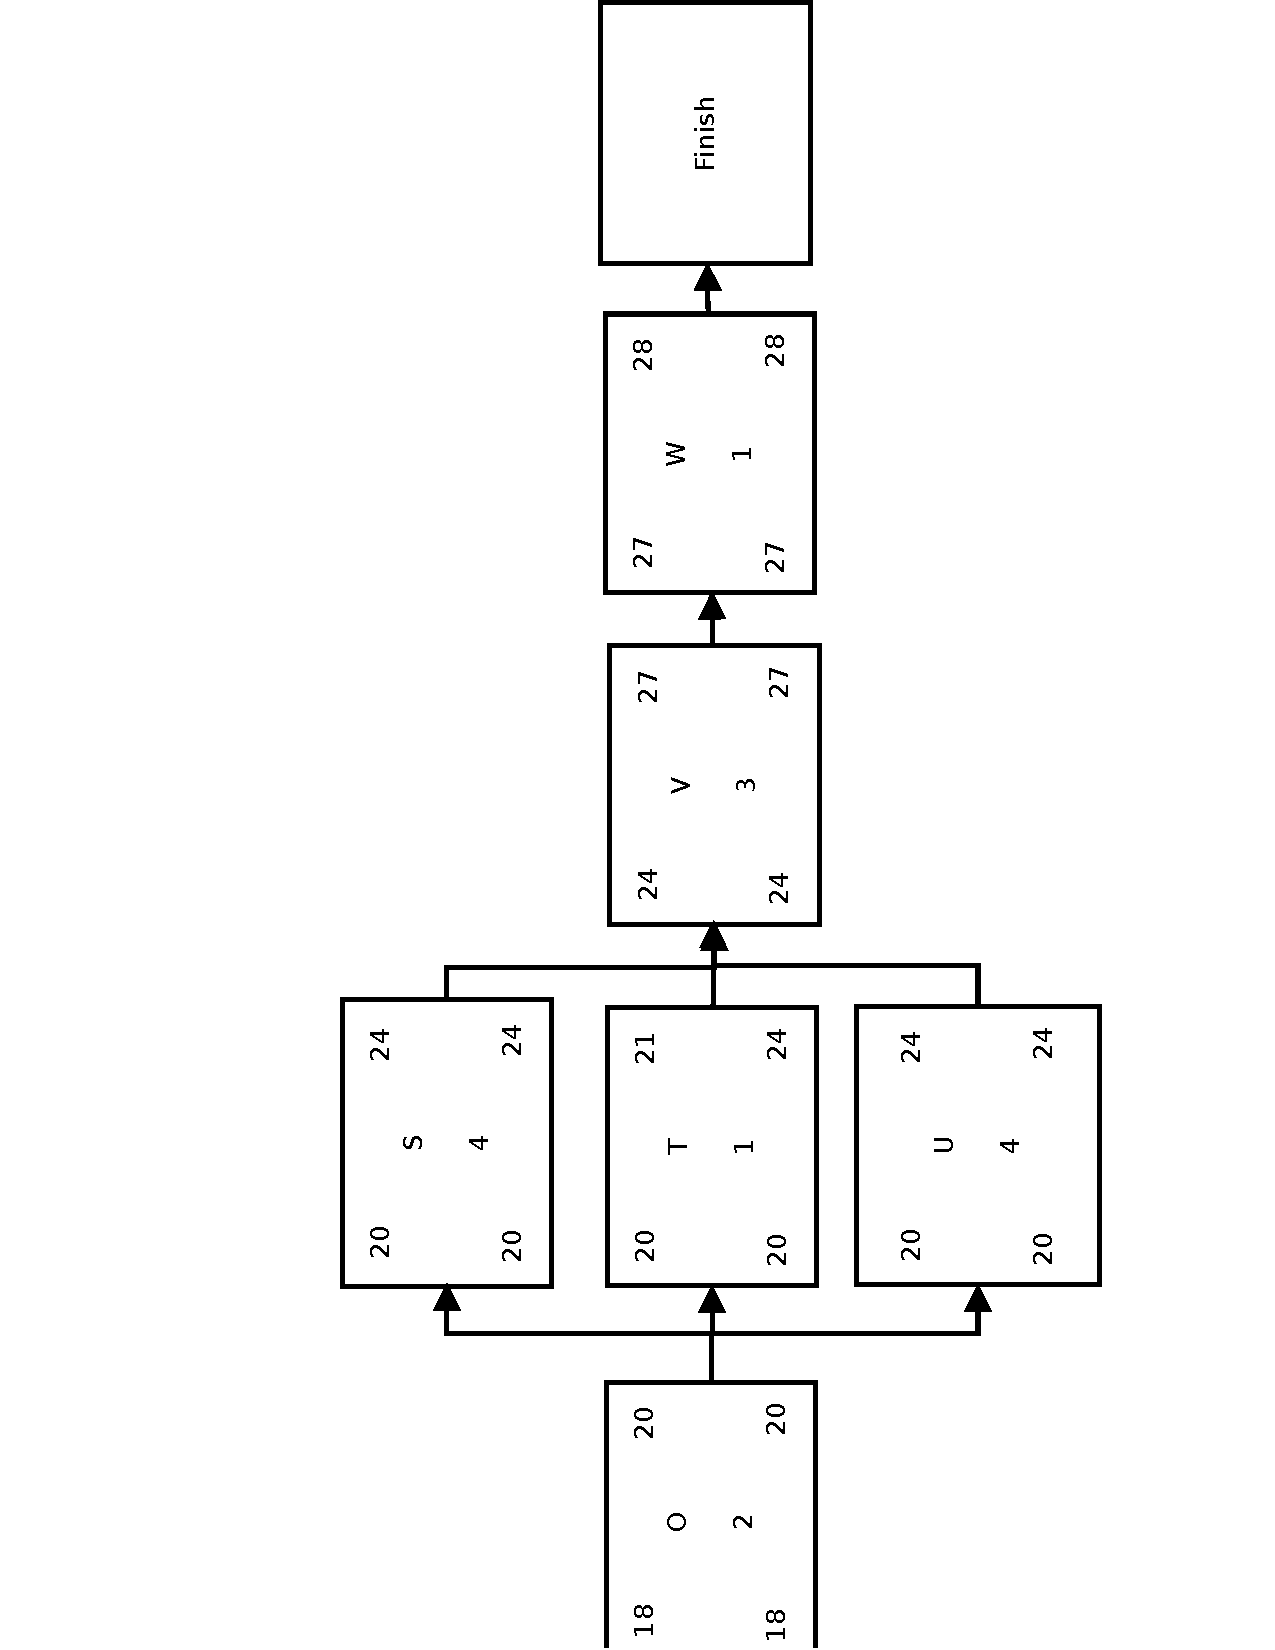
\includegraphics[scale=0.6]{figures/hw5-pdm-3}
    \end{subfigure}
    \label{figure:pdm}
\end{figure}
% continued
\begin{figure}
    \ContinuedFloat % continue from previous page
    \begin{subfigure}{\textwidth}
        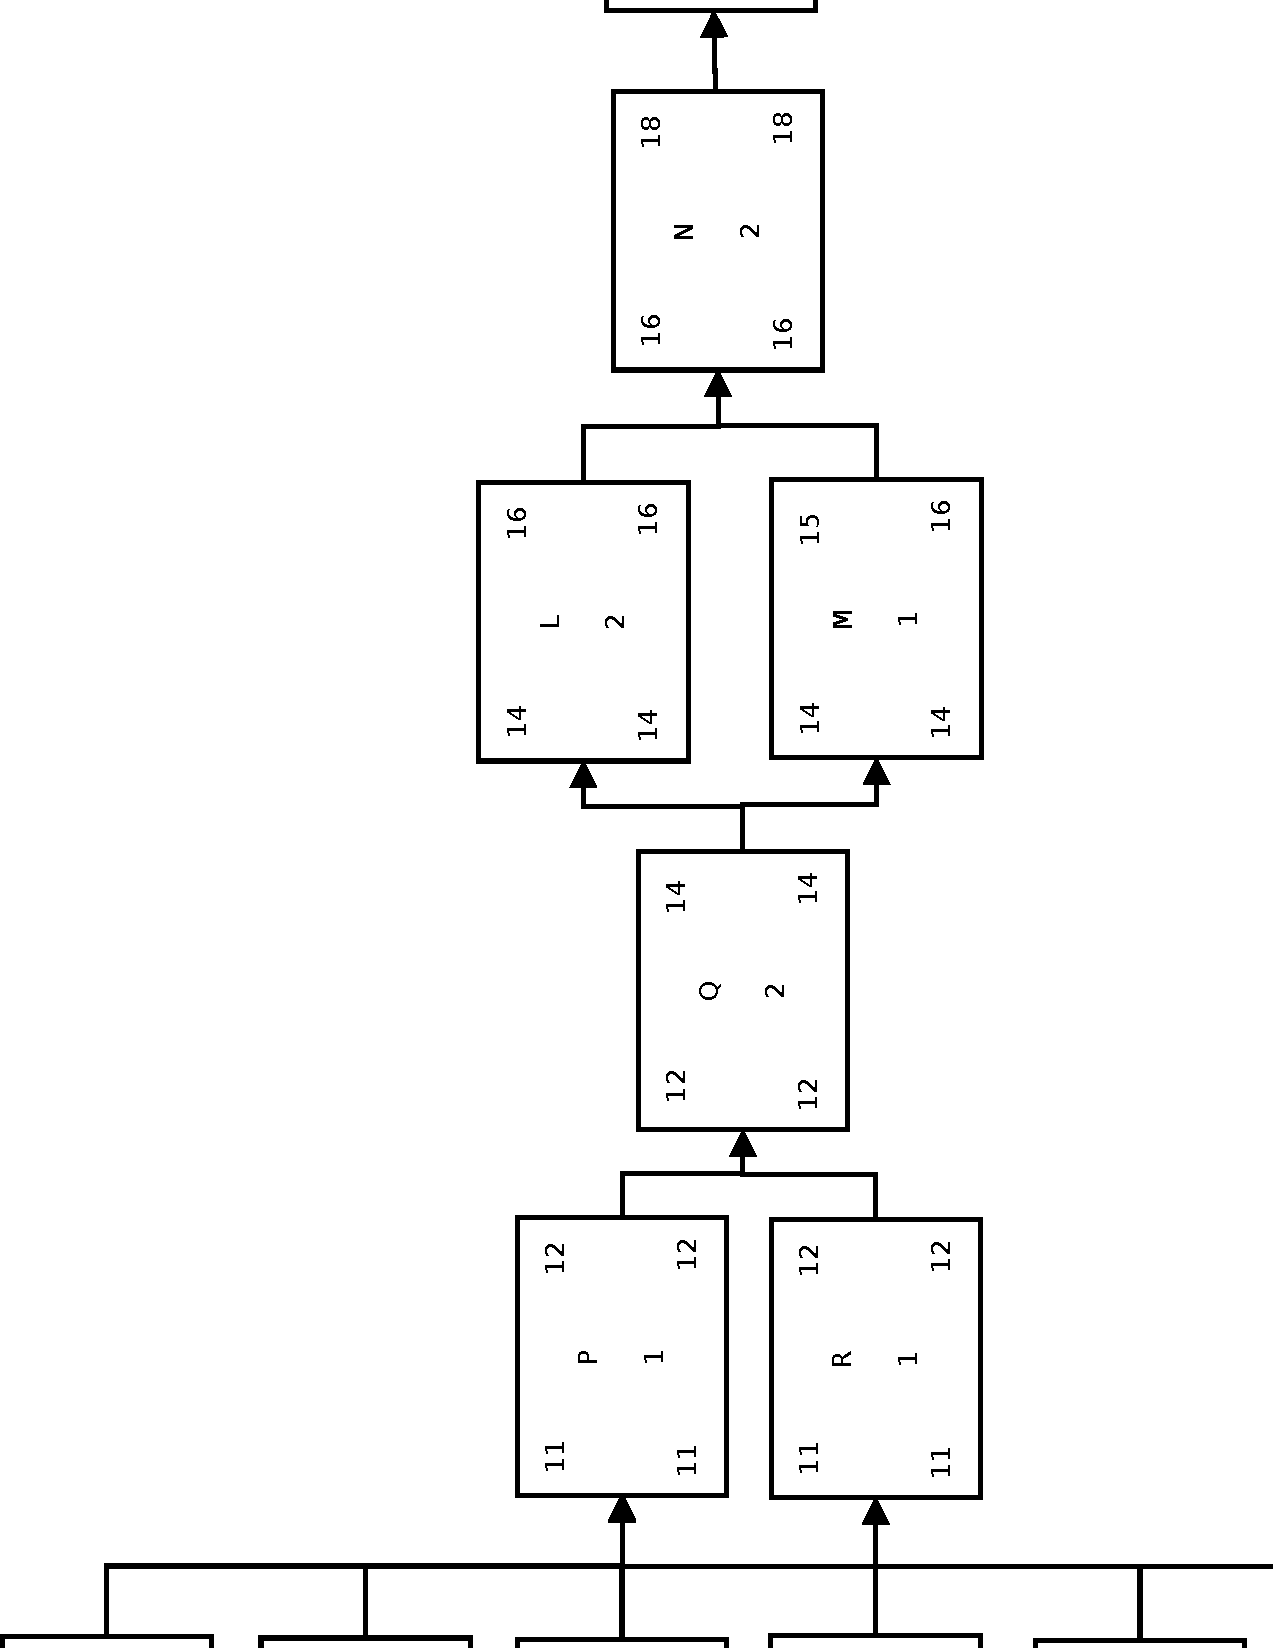
\includegraphics[scale=0.6]{figures/hw5-pdm-2}
    \end{subfigure}
\end{figure}
% continued
\begin{figure}
    \ContinuedFloat % continue from previous page
    \begin{subfigure}{\textwidth}
        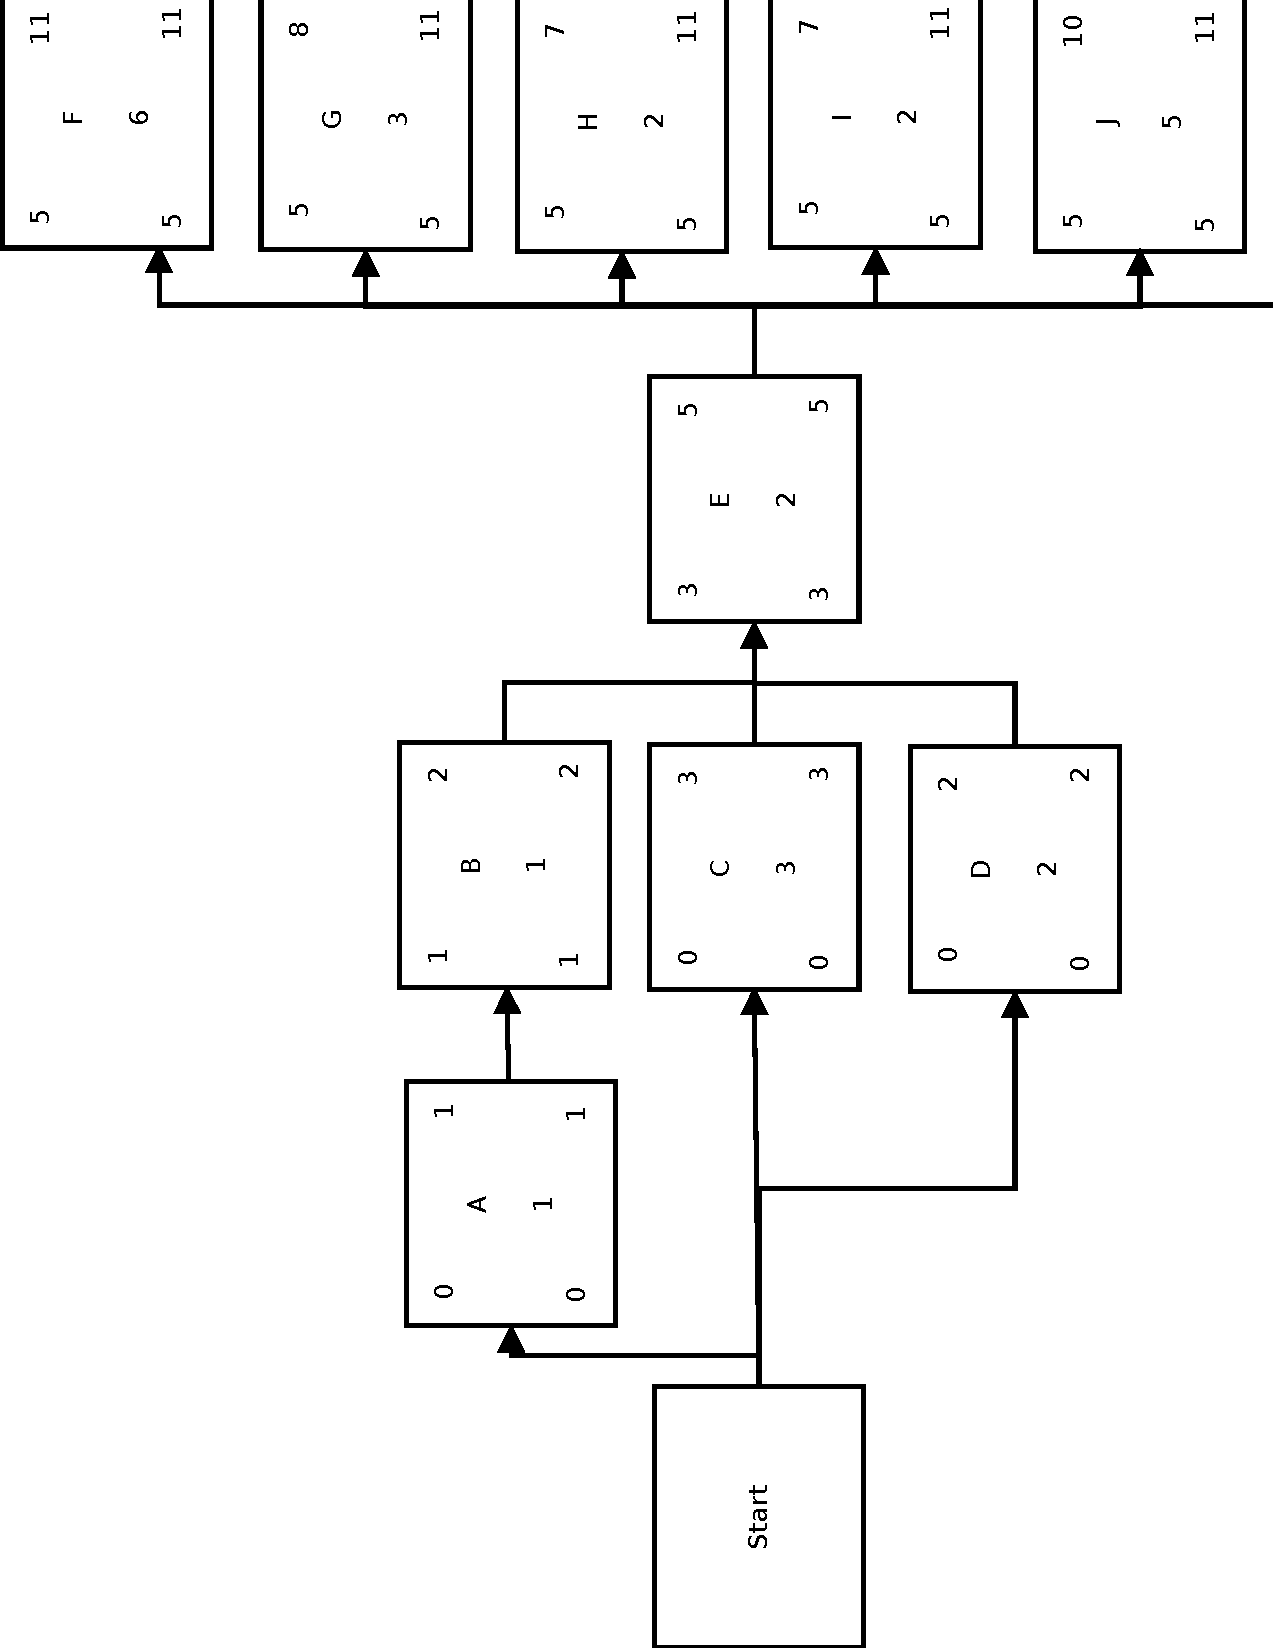
\includegraphics[scale=0.6]{figures/hw5-pdm-1}
    \end{subfigure}
\end{figure}
